\section{Controlled Robustness Analysis}
\label{sec:robustness}
%---------------------------------------------------------------------

This section examines sensitivity to incomplete inputs, additive
Gaussian perturbations, and synthetic feature scaling. These
experiments complement clean classification and calibration analysis
but do not establish reliability under field conditions.

The results originate from earlier saved noncompact model
configurations. They are distinct from the compact five-seed comparison
reported in Section~\ref{sec:experimental_results}. Robustness
measurements have not been regenerated for those compact models;
therefore, the present findings are not attributed to their compact
embeddings, anchored knowledge policy, or controlled training objective.

Two missing-input experiments are reported separately: a
cross-model zero-replacement experiment and a within-model imputation
comparison. Their clean reference accuracies differ because they use
different saved-model evaluations. Results are compared within each
experiment rather than combined into a single configuration ranking.

%---------------------------------------------------------------------
\subsection{Perturbation Protocols}
%---------------------------------------------------------------------

\subsubsection{Random Feature Masking}

Let $\mathbf{z}_i\in\mathbb{R}^{7}$ denote a standardized
evaluation input. For masking probability
$m\in\{0,0.2,0.4,0.6\}$, each feature is independently selected
for masking:

\begin{equation}
b_{i,j}^{(t)}
\sim
\operatorname{Bernoulli}(m),
\label{eq:robustness_mask}
\end{equation}

where $t$ denotes the perturbation trial. Thus, $m$ is the
probability of masking an individual feature entry, not an exact
fraction of features removed from every record.

The cross-model experiment replaces masked entries with zero:

\begin{equation}
\widetilde{z}_{i,j}^{(t)}
=
\begin{cases}
0, & b_{i,j}^{(t)}=1,\\
z_{i,j}, & b_{i,j}^{(t)}=0.
\end{cases}
\label{eq:robustness_zero_fill}
\end{equation}

Because the inputs are standardized, zero represents the corresponding
training-feature mean. This experiment therefore measures sensitivity
to random mean replacement rather than native missing-value handling.

The evaluation routine uses a pseudorandom generator initialized with
seed 42 and five trials per masking level. Each classifier receives
the same perturbation sequence within this cross-model experiment.

\subsubsection{Training-Derived Imputation}

A separate experiment represents masked entries as NaNs and compares
zero replacement, median imputation, five-neighbor KNN imputation,
and iterative imputation for the same evaluated KG-Hybrid checkpoint.

All imputers are fitted on the standardized training partition and
applied to incomplete test inputs without refitting. The iterative
imputer uses random state 42 and at most ten iterations. Within each
trial, all recovery methods receive the same missing-entry mask.

Five trials are averaged at each masking probability. The saved
aggregate results do not provide trial-level standard deviations;
therefore, confidence intervals and significance claims are not
assigned to these robustness measurements.

\subsubsection{Additive Gaussian Perturbations}

Gaussian perturbations are applied to standardized evaluation inputs:

\begin{equation}
\widetilde{\mathbf{z}}_i^{(t)}
=
\mathbf{z}_i+\boldsymbol{\epsilon}_i^{(t)},
\qquad
\boldsymbol{\epsilon}_i^{(t)}
\sim
\mathcal{N}(\mathbf{0},\sigma^2\mathbf{I}_7),
\label{eq:robustness_noise}
\end{equation}

with $\sigma\in\{0,0.1,0.2,0.3\}$. The routine uses seed 42
and five perturbation trials per noise level.

The noise magnitudes are expressed in standardized feature
coordinates. They do not denote a common physical error magnitude
across nutrient, temperature, humidity, pH, and rainfall measurements.

\subsubsection{Synthetic Feature Scaling}

The feature-scaling experiment applies

\begin{equation}
\widetilde{\mathbf{z}}_i
=
1.5\mathbf{z}_i
\label{eq:robustness_scaling}
\end{equation}

while retaining the original benchmark labels. In original feature
coordinates, this corresponds to increasing displacement from the
training mean, rather than multiplying every raw measurement by 1.5.

This transformation does not guarantee that every feature moves
outside its observed training range. Accordingly, it is described
as synthetic feature scaling rather than verified out-of-range
extrapolation or cross-dataset validation.

For masking and noise, reported accuracy is the arithmetic mean
over five trials:

\begin{equation}
\overline{A}
=
\frac{1}{5}
\sum_{t=1}^{5}
\frac{1}{N}
\sum_{i=1}^{N}
\mathbf{1}
\left[
\hat{y}_i^{(t)}=y_i
\right].
\label{eq:robustness_average}
\end{equation}

The deterministic feature-scaling experiment uses a single
transformed evaluation partition.

%---------------------------------------------------------------------
\subsection{Sensitivity to Missing Inputs}
%---------------------------------------------------------------------

\subsubsection{Cross-Model Zero-Replacement Results}

Fig.~\ref{fig:results_missing_features} reports the recorded cross-model
masking results.



Accuracy decreases for every model as masking increases.
At 40\% masking, KG-Hybrid obtains 53.27\% accuracy,
compared with 65.64\% for XGBoost, 60.30\% for
Random Forest, and 48.12\% for FT-Transformer.

XGBoost achieves the highest recorded accuracy at every nonzero
masking level. KG-Hybrid exceeds FT-Transformer under this protocol
but does not outperform the tree baselines. The results therefore
do not support a general missing-input robustness advantage for
the integrated architecture.

\subsubsection{Within-Model Imputation Results}

Fig.~\ref{fig:robustness_imputation} presents the separate
within-model recovery comparison. All recovery methods use the same evaluated
KG-Hybrid checkpoint and have the same clean reference accuracy
of 97.88\%.

\begin{figure}[t]
\centering
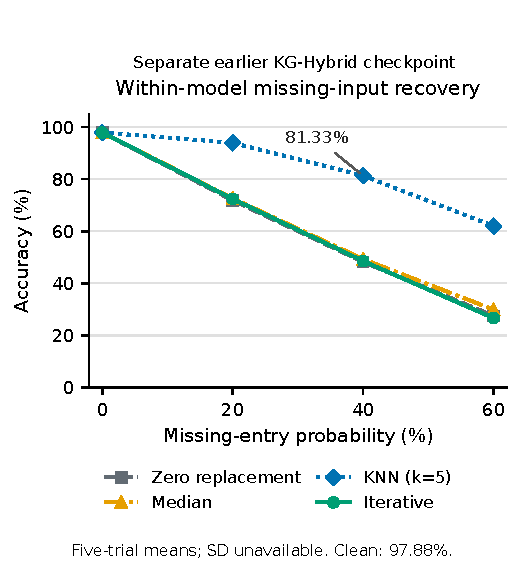
\includegraphics[width=\columnwidth]
{table_replacement_figures/table_xi_imputation.pdf}
\caption{Earlier within-model KG-Hybrid imputation comparison.
Points show mean accuracy over five trials using a separate
checkpoint with clean accuracy 97.88\%.
All recovery methods share the same missing-entry mask within
each trial, and imputers are fitted on standardized training data.
Trial-level standard deviations are unavailable.
The checkpoint differs from that evaluated in
Fig.~\ref{fig:results_missing_features}.}
\label{fig:robustness_imputation}
\end{figure}

At 40\% masking, KNN imputation increases recorded accuracy
from 48.24\% under zero replacement to 81.33\%, a
difference of 33.09 percentage points. It also exceeds the
median and iterative imputation results in this experiment.

At 60\% masking, KNN-based accuracy decreases to 61.94\%.
Recovery therefore mitigates the measured degradation but does
not restore clean-input performance under severe information loss.

This comparison supports a protocol-specific benefit of
training-derived KNN imputation for the evaluated checkpoint.
It does not establish that the knowledge-guided architecture
is responsible for the benefit or that similarly imputed
baseline classifiers would perform worse. Equivalent
imputation-controlled comparisons are not available for every
baseline.

%---------------------------------------------------------------------
\subsection{Sensitivity to Gaussian Perturbations}
%---------------------------------------------------------------------

Fig.~\ref{fig:results_noise} reports the recorded noise
experiment using standardized inputs.



At $\sigma=0.2$, KG-Hybrid achieves 80.97\% accuracy.
This exceeds XGBoost by 1.27 percentage points but remains
below Random Forest and FT-Transformer.

At $\sigma=0.3$, KG-Hybrid obtains 67.15\%, below
XGBoost at 68.36\%, Random Forest at 75.64\%, and
FT-Transformer at 78.85\%. Its decrease from the clean
reference is 32.55 percentage points.

FT-Transformer achieves the highest recorded accuracy at each
nonzero noise level. These findings do not establish a Gaussian-noise
robustness advantage for KG-Hybrid and do not identify any
individual architectural component as the cause of its behavior.

The experiment considers independent additive Gaussian noise only.
It does not assess systematic bias, correlated errors, outliers,
sensor drift, or feature-dependent physical measurement tolerances.

%---------------------------------------------------------------------
\subsection{Sensitivity to Synthetic Feature Scaling}
%---------------------------------------------------------------------

Fig.~\ref{fig:results_scaling} reports results after multiplying
standardized test vectors by 1.5.



FT-Transformer obtains the highest recorded accuracy,
92.12\%. KG-Hybrid achieves 82.42\%, below XGBoost
at 83.33\% and above Random Forest at 80.00\%.

The scaling results differ from the clean-data ranking,
illustrating that strong benchmark accuracy does not ensure
stability under synthetic input displacement. However, the
transformation is not evidence of geographical or seasonal
generalization.

All perturbed inputs retain their original crop labels.
Whether those labels remain agronomically appropriate after
the transformation has not been established. The measured
accuracy therefore quantifies preservation of benchmark
predictions, not validated crop suitability under changed
environmental conditions.

%---------------------------------------------------------------------
\subsection{Predictive Variability: Implementation and Scope}
%---------------------------------------------------------------------

The inference implementation additionally supports predictive
variability estimation using $M=10$ MC-Dropout passes.
This mechanism is distinct from the deterministic perturbation
accuracy experiments above.

For class $c$, the implementation computes

\begin{equation}
\overline{p}_c
=
\frac{1}{M}
\sum_{t=1}^{M}p_c^{(t)}
\label{eq:robustness_mc_mean}
\end{equation}

and the population standard deviation

\begin{equation}
s_c
=
\sqrt{
\frac{1}{M}
\sum_{t=1}^{M}
\left(p_c^{(t)}-\overline{p}_c\right)^2
}.
\label{eq:robustness_mc_std}
\end{equation}

The reported crop and variability score are

\begin{equation}
\hat{c}
=
\arg\max_c \overline{p}_c,
\qquad
s_{\mathrm{pred}}=s_{\hat{c}}.
\label{eq:robustness_variability}
\end{equation}

Thus, the reported variability is the standard deviation for
the predicted class, not the maximum standard deviation
across all classes.

Only explicit dropout modules are activated during stochastic
inference. In the full Transformer configuration, attention
modules remain in evaluation mode, so their internal
attention-weight dropout is not activated by this procedure.

The resulting score measures variability under the implemented
dropout mechanism. It is not a calibrated probability of error,
a complete uncertainty estimate, or a measure of physical
agricultural risk. The robustness experiments do not establish
its error-detection performance or whether it reliably increases
with perturbation severity.

XGBoost fast-path predictions do not undergo MC-Dropout sampling.
A zero variability field returned on that path denotes an
uncomputed estimate rather than evidence of zero uncertainty.

%---------------------------------------------------------------------

Broader limitations and future validation requirements are discussed
in Section~\ref{sec:limitations}.

